% ============================================================================================
% Verifier Economics --- MASTER MANUSCRIPT (Paper D of the InceptLabs self-improvement family).
% This is the complete, format-neutral, self-contained version. Conference-format cuts are derived
% from it (see verifier_economics-AAAI.tex). Build: tectonic verifier_economics.tex
% Figures from make_figs.py (figs/*.pdf). Every headline number is from rna_harness/runs/*.
% ============================================================================================
\documentclass[11pt]{article}
\usepackage[margin=1in]{geometry}
\usepackage{amsmath,amssymb,amsthm}
\usepackage{booktabs}
\usepackage{graphicx}
\usepackage{xcolor}
\usepackage{array}
\usepackage[hidelinks]{hyperref}
\usepackage{natbib}
\usepackage{caption}
\captionsetup{font=small,labelfont=bf}
\emergencystretch=1.5em

\newtheorem{theorem}{Theorem}
\newtheorem{proposition}{Proposition}
\newcommand{\match}{\ensuremath{\mathcal{A}_{\mathrm{match}}}}
\newcommand{\umfe}{\ensuremath{\mathcal{A}_{\mathrm{uMFE}}}}
\newcommand{\pfe}{\ensuremath{\mathcal{A}_{\mathrm{pfe}}}}
\newcommand{\PT}{\ensuremath{P(T)}}

\title{\textbf{``Solved'' Is a Purchase, Not a Fact}\\[2pt]
\large Deterministic Cost--Robustness Frontiers of Verifier Choice in RNA and SAT}
\author{Wenhui Chen \quad The Verifier-Economics Team\\ InceptLabs-Shanghai}
\date{2026 \quad\textit{(complete manuscript; conference-format versions derived separately)}}

\begin{document}
\maketitle

\begin{abstract}
\noindent A cost-optimal RNA designer, judged by the standard folding oracle it must project its
pseudoknotted targets onto, appears to solve \textbf{250 of 251} of them; judged by an oracle that can
represent the crossing pairs, essentially none of those designs form the true target. That $99.6\%$
``solved'' rate is an artifact of \emph{which verifier one can afford to run}. This is the thesis of the
paper. The prevailing response to noisy reward models in reinforcement learning with verifiable rewards
(RLVR) is to make the verifier \emph{deterministic}---executable tests, symbolic checkers, folding
oracles---on the premise that a computed verdict cannot be reward-model error. We argue determinism is
\emph{necessary but not sufficient}: even a fully \emph{decidable} verifier over-accepts on two orthogonal
axes---using the \emph{wrong oracle} (one that cannot represent the objective) and using a \emph{too-weak
rung} (one whose criterion is satisfiable without the property one cares about). ``Solved'' is thus not a
property of a solution but a \emph{choice of verifier}, and that choice trades cost against robustness along
a frontier that---because the verifiers in wide use are noisy and offer no strength knob---is usually argued
rather than measured. We contribute the \emph{instrument} to measure it: we turn RNA secondary-structure
inverse design and Boolean satisfiability
into a \emph{deterministic, dial-able, cost-priced} verifier testbed in which a single problem admits a
strictly ordered family of \emph{decidable} predicates whose verdict is \emph{computed}, not judged: for
RNA, exact-match $\supseteq$ unique-MFE $\supseteq$ target Boltzmann probability $\ge\theta$ (a provable
nesting for $\theta>\tfrac12$), with pseudoknots forming a separate oracle \emph{branch}. We establish four
results; the over-acceptance and cost findings are mirrored in SAT (so they are properties of cheap-proxy
verification, not of RNA), while the Goodhart effect is domain-dependent and carried by RNA.
\textbf{(1)}~Verifiers over-accept on two axes: an out-of-domain oracle, reached by specification
projection, false-accepts almost everything ($99.6\%$), and a too-weak rung on the right
oracle lets $92\%$ of exact-match ``solutions'' collapse under an ensemble-robustness verifier, with
fragility growing in hardness (mirrored in SAT). \textbf{(2)}~Optimizing the cheap proxy Goodharts
robustness: with the proposer fixed and only the reward varied, strong-reward robust-acceptance climbs with
budget ($12\%\!\to\!33\%$) while cheap-reward does not ($18\%\!\to\!16\%$), separating with disjoint
confidence intervals. \textbf{(3)}~The cost of strictness depends on computation reuse: a small constant
($\sim\!4\times$) in RNA, where the strong rung amortizes the cheap oracle's work, but steep
($\sim\!400\times$) in SAT, where it needs a neighborhood scan. \textbf{(4)}~Nesting yields a provably
\emph{sound} ($\epsilon{=}0$) cheapest-first routing cascade,
yet a finite-sample risk analysis shows the cheap rungs so gameable ($\min\epsilon{=}0.999$) that certifying
robustness is near-incompressible. Finally, on real LLM code verifiers (four models) the over-acceptance
reproduces---$7.5$--$9.2\%$ of programs passing weak provided tests fail a held-out population---and,
validating dial-ability, strengthening the cheap rung monotonically cuts that mass (to $0$--$5\%$) in every
model, with the Goodhart divergence appearing under optimization in the weaker models. All verdicts are
relative to a declared computational model. The contribution is the \emph{instrument}, not a new phenomenon: a place to measure the verifier
problem exactly.
\end{abstract}

\section{Introduction}\label{sec:intro}
Reinforcement learning with verifiable rewards (RLVR) has moved the binding constraint of large-model
training away from compute and onto the \emph{verifier} \citep{verificationhorizon,hiddencosts}. A reward
signal must satisfy three requirements simultaneously: it must be \emph{cheap} enough to evaluate at the
scale of millions of rollouts, \emph{faithful} enough that improving it improves the true objective, and
\emph{robust} enough that an optimizer cannot satisfy its letter while violating its intent. Achieving all
three at once is widely reported to be unsolved. When the reward is an imperfect proxy, optimization
Goodharts the true objective: models discover shortcuts that pass an \emph{extensional} check (does this
output look right?) while failing an \emph{intensional} one (is it right for the right reason?), and the
prevalence of such shortcuts rises with optimization pressure \citep{gamingverifiers,rubricrewardhacking,
correlatedproxies}.

The verifiers in which this has been studied---LLM judges, learned rubric models, unit-test suites, and
deliberately hackable environments \citep{hackverifiable}---share two properties that make the
cost--robustness tension impossible to measure cleanly. They are \emph{noisy}: the same output can receive
different verdicts, so any measured gap between a weak and a strong verifier is confounded by evaluator
variance. And they are \emph{not dial-able}: there is no knob that turns a verifier continuously from
``cheap and permissive'' to ``expensive and strict'' while holding everything else fixed. As a result the
tension is discussed qualitatively---stronger verifiers are ``better but costlier''---but never quantified
as a frontier one can trade along.

\paragraph{A running example.} Consider designing an RNA sequence that folds into a target
\emph{pseudoknotted} structure---one whose base pairs cross, a motif central to many functional RNAs. The
default, ubiquitous tool (ViennaRNA's minimum-free-energy folding) cannot represent crossing pairs at all.
A practitioner who nonetheless uses it is \emph{forced} to optimize toward the target's nested
\emph{skeleton}---and the tool will report ``solved'' on that skeleton. We ran exactly this on $251$ natural
pseudoknots: the blind tool certifies the skeleton for $250$ of them, while a pseudoknot-aware predictor
finds the crossing stem the true target requires forms in \emph{none}. Relative to the real objective,
$250/251$ ``solved'' designs are false accepts. The design did not get better or worse; the \emph{verifier}
changed---specifically, the objective was silently projected onto what the affordable oracle can see---and
with it the answer to ``is this solved?'' went from $99.6\%$ to nearly zero. This is not a corner case: it
is the generic hazard whenever the verifier one can afford is blind to part of the objective and nothing
forces it to abstain.

\paragraph{This paper.} The common defense against reward hacking is to replace a learned reward model with
a \emph{deterministic} verifier---unit tests, symbolic answer-checking, a folding oracle---on the premise
that a computed verdict has no reward-model error to exploit \citep{verificationhorizon}. Our central claim
is that determinism is \emph{necessary but not sufficient}: a fully \emph{decidable} verifier can still be
gamed, on two orthogonal axes that determinism does nothing to close---choosing an oracle that cannot
represent the objective (Axis~1), and choosing a rung whose criterion is met without the property one
actually wants (Axis~2). We argue, in short, that ``solved'' is not a property of a solution but a
\emph{choice of verifier}, and we build a testbed where that choice becomes a measurable, controllable
variable. We use two unrelated \emph{deterministic} domains---RNA inverse design and Boolean satisfiability
(SAT)---in which a single problem admits a strictly ordered family of \emph{decidable} acceptance
predicates: their verdict is
\emph{computed} by a fixed algorithm, not judged, so there is zero evaluator variance, and they can be
\emph{dialed} from a cheap permissive proxy to an expensive strict predicate, each with a measurable cost.
This lets us measure, exactly, how the gap between what a cheap verifier accepts and what a strong verifier
accepts moves with verifier strength, problem hardness, and optimization pressure; and it lets us
\emph{prove} and finite-sample-calibrate policies for routing candidates through the ladder. Throughout,
``solved'' means solved under a declared computational folding/energy model---a model-relative verdict,
which is exactly the regime in which every practical verifier already operates.

\paragraph{Contributions.}
\begin{enumerate}\itemsep2pt
\item A deterministic, dial-able, cost-priced verifier ladder in two natural domains (RNA, SAT), with a
proved strictness nesting and an explicit treatment of out-of-domain oracles as a \emph{branch}
(\S\ref{sec:ladder}).
\item An experimental protocol and cost model that make ``how strong is this verifier, and what did it
cost?'' a measurable quantity (\S\ref{sec:setup}).
\item A cross-domain measurement of verifier over-acceptance along \emph{two independent axes}---using the
wrong oracle ($99.6\%$ false positives) and using a too-weak rung on the right oracle ($92\%$ collapse)---
and of how both worsen with problem hardness (\S\ref{sec:gap}).
\item A controlled, RL-free demonstration that optimizing the cheap proxy Goodharts a robustness objective,
with the effect attributed to the verifier alone (\S\ref{sec:goodhart}).
\item An end-to-end cost accounting showing the price of strictness is governed by computation reuse---a
small constant in RNA (shared partition-function pass) but steep in SAT (Hamming-ball scan) (\S\ref{sec:cost}).
\item A provably sound ($\epsilon{=}0$) cheapest-first routing cascade, plus a finite-sample risk analysis
showing that relaxing onto cheaper rungs is nearly impossible without accepting massive false-positive
rates---a quantified, near-incompressible cost of robustness (\S\ref{sec:routing}).
\item A validation that both mechanisms transfer to the target domain---a real LLM code verifier---where
weak provided tests over-accept and cheap-proxy optimization fails to build held-out robustness while
strong-rung optimization does (\S\ref{sec:llm}).
\end{enumerate}
\S\ref{sec:discussion} draws the implications for reward design; \S\ref{sec:related} positions the work.

\section{The Verifier as a Graph: A Nested, Priced Ladder}\label{sec:ladder}
The central object is not a single verifier but a \emph{family} of them over one problem, partially ordered
by strictness and partitioned by which oracle (structure model) they use. Figure~\ref{fig:ladder} shows the
shape: within one oracle the predicates nest, and a structure class the oracle cannot represent is a
separate branch reachable only by changing oracles.

\begin{figure}[t]\centering
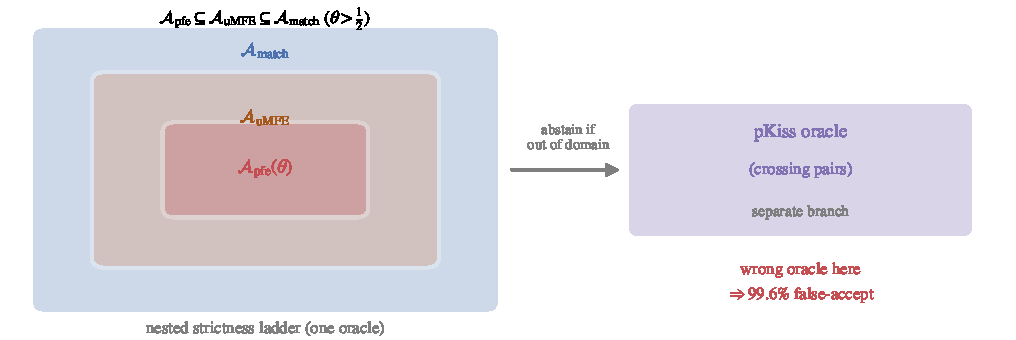
\includegraphics[width=0.92\linewidth]{figs/f0_ladder.pdf}
\caption{The verifier as a \emph{graph}, not a scalar. Within one oracle, strictness forms a nested ladder
($\match{}\supseteq\umfe{}\supseteq\pfe{}$); an out-of-domain structure class (pseudoknots) is a separate
\emph{branch} with its own oracle (pKiss), \emph{not} a superset of the first. Treating a wrong-oracle
target as a rung---rather than abstaining---is precisely what produces the $99.6\%$ false-accept rate of
\S\ref{sec:gap}.}\label{fig:ladder}
\end{figure}

\subsection{RNA (pseudoknot-free)}
A candidate is a sequence $x\in\{A,C,G,U\}^n$; a target $T$ is a dot-bracket secondary structure. Fix a
thermodynamic model (ViennaRNA, Turner~2004 parameters, $37^\circ$C) \citep{lorenz2011viennarna}. We define
three acceptance sets over $x$, in increasing strictness:
\begin{itemize}\itemsep1pt
\item \match{}$=\{x:\mathrm{MFE}(x)=T\}$: the sequence's minimum-free-energy structure equals $T$. This is
the cheap proxy---the most common ``solved'' criterion in RNA-design benchmarks, though robustness-aware
objectives (unique MFE, ensemble defect, probability defect) are also long established
\citep{zadeh2011nupack,zhou2023samfeo}.
\item \umfe{}$=\{x:T\text{ is the \emph{unique} MFE of }x\}$: $T$ is the sole ground state, closing the
degenerate-co-optimal loophole in which several structures tie for lowest energy.
\item \pfe{}$(\theta)=\{x:\PT{\mid}x\ge\theta\}$: the target's Boltzmann probability in the pseudoknot-free
ensemble clears a threshold---a \emph{robust} fold, not a fragile one-of-many.
\end{itemize}
These are decidable, and for a suitable threshold they nest:
\begin{equation}\label{eq:nest}
\pfe(\theta)\ \subseteq\ \umfe\ \subseteq\ \match,\qquad \theta>\tfrac12 .
\end{equation}
The bound $\theta>\tfrac12$ is both necessary and sufficient for the first inclusion (Proposition~\ref{prop:nest},
Appendix~\ref{app:proofs}); below it, \pfe{} is only a threshold family, not a stronger rung. Empirically
the nesting holds exactly: $0$ violations over the $304$ solved solutions of \S\ref{sec:gap}.

\subsection{Pseudoknots are a branch, not a rung}
On a pseudoknotted target, ViennaRNA cannot emit crossing pairs, so \match{}/\umfe{}/\pfe{} are
\emph{inapplicable}, not merely weaker. A pseudoknot-aware oracle (pKiss \citep{janssen2015pkiss}) uses a
different structure space and heuristic, and its acceptance set is \emph{not} a superset of the Vienna one.
The correct object is therefore a verifier \emph{graph}: a nested strictness branch per representable
structure class, together with a \emph{domain-of-validity gate} that \emph{abstains} when the oracle is out
of domain, rather than silently accepting a projected (skeleton) target. The distinction is not pedantic:
\S\ref{sec:gap} shows that ignoring it converts an oracle into a near-perfect false-positive generator.

\subsection{SAT (the mirror domain)}
A candidate is an assignment $x$ to a CNF formula $\varphi$. The cheap rung is $V_0=\{x:\varphi(x)=\text{true}\}$.
A continuous robustness measure $\rho(x)$ is the fraction of single-variable flips of $x$ that remain
satisfying; the strong rungs are $\{x:\rho(x)\ge\theta\}\subseteq V_0$, and a radius-$r$ generalization
requires satisfaction throughout a Hamming ball of radius $r$. Hardness is the clause density $\alpha=m/n$,
with the random 3-SAT threshold at $\alpha_c\approx4.267$. That satisfying assignments become fragile and
clustered as $\alpha\to\alpha_c$ (frozen variables, shattered solution space) is classical statistical
physics \citep{krzakala2007clustering,zhou2008frozen}; we reuse it as a decidable strong rung, not as a new
notion. SAT shares no mechanism with RNA folding, so any phenomenon that appears in both is a property of
cheap-proxy verification itself.

\section{Experimental Setup}\label{sec:setup}
\paragraph{Benchmarks.} The RNA frontier and Goodhart experiments use EteRNA100-V2 \citep{eterna100v2}:
$100$ community-designed targets spanning $12$--$400$\,nt. The wrong-oracle study uses $251$ natural
pseudoknots from Pseudobase++ ($21$--$137$\,nt, with $3$--$57$ crossing pairs). SAT uses random 3-CNF
formulas at clause densities $\alpha\in\{3.0,3.4,3.8,4.0,4.2,4.267,4.4,4.6\}$ spanning the satisfiability
threshold, with $k=40$ instances per density; for the robustness frontier we set $n=14$ and enumerate all
$2^{14}$ assignments per formula, so satisfiability and solution-set robustness are computed exactly with
no solver in the loop (\S\ref{sec:axis2}).

\paragraph{Model of ``solved.''} All RNA verdicts use ViennaRNA~2.7.2 with Turner~2004 parameters,
$37^\circ$C, and \texttt{dangles=2}; \pfe{} uses the partition function with $\theta=0.9$. Pseudoknotted
targets are judged by pKiss. SAT verdicts are exact: $\varphi(x)$ for $V_0$, and $\rho(x)$ by enumerating
all single-variable flips. Every verdict is model-relative---``solved'' means solved under the declared
computational model, never a claim about in-vivo biology (\S\ref{sec:limits}).

\paragraph{The cost-optimal solver (the ``agent'').} To produce candidates that a cheap verifier would
accept, we run a replica-exchange Monte-Carlo (REMC) search that optimizes \emph{only} the cheap proxy to
$\mathrm{bp}=0$: eight replicas on a geometric temperature ladder with adjacent-replica swaps, a structural
warm-start, and a defect-cluster ``endgame'' for last-mile repair, under a $30$\,s wall budget per target.
SAT candidates come from a WalkSAT-style local search. This is deliberately a \emph{proxy-optimizer}: it is
the stand-in for an RL policy that has learned to satisfy the reward it is given. We draw $5$ independent
solver seeds per target, so every headline rate carries a bootstrap confidence interval over
seed$\times$target units. Solver internals and pseudocode are in Appendix~\ref{app:methods}.

\paragraph{Cost model.} Each rung is priced by its end-to-end verification cost---wall-clock time from the
raw pair $(x,T)$ to an accept/reject verdict, measured in-process with warm caches, reported as a median
over repetitions ($15$ for RNA, $25$ for SAT). We report milliseconds; the currency generalizes additively
to solver CPU-seconds and, for an LLM verifier, to tokens, all on one axis.

\paragraph{Statistics.} Rates carry bootstrap $95\%$ confidence intervals ($B=5000$ resamples over
seed$\times$target units). False-positive rates carry one-sided Clopper--Pearson \citep{clopperpearson1934}
upper bounds at confidence $1-\delta$ ($\delta=0.05$). The nesting check counts, per solution, any rung pair
that violates Eq.~\eqref{eq:nest}.

\section{The Verifier Gap: Two Axes of Over-Acceptance}\label{sec:gap}
A verifier can over-accept---call a bad solution good---in two independent ways: by using the \emph{wrong
oracle}, one that cannot even represent the objective, or by using a \emph{too-weak rung} on the right
oracle. The two axes are orthogonal and both are severe; we measure each in turn.

\subsection{Axis 1: an out-of-domain oracle via specification projection ($99.6\%$)}\label{sec:axis1}
We instantiate the running example of \S\ref{sec:intro} at scale, and we are careful about what is
measured. ViennaRNA cannot represent crossing pairs at all, so to use it on a pseudoknotted target a
practitioner is \emph{forced} to project the target onto its nested skeleton. We quantify the cost of that
projection. For each of $251$ natural pseudoknots the cost-optimal search designs against the skeleton;
the pseudoknot-blind harness then certifies \textbf{$250$ of $251$} designs as ``solved''---their skeleton
is indeed the MFE. (The one exception, a $4$-crossing-pair target, the search could not skeleton-solve, so
it was never claimed.) We then ask a pseudoknot-aware \emph{predictor}---pKiss under a fixed configuration,
a heuristic over a restricted pseudoknot class, not a biophysical gold oracle---whether the \emph{full}
target forms: it predicts the required crossing stem forms in $\mathbf{0}$ of the $250$
(Table~\ref{tab:pk}, Table~\ref{tab:pkcontingency}, Figure~\ref{fig:pk}). The false-accept rate relative to
the true, unprojected target is therefore $250/251=99.6\%$, and it is \emph{flat across complexity}:
$60/61=98\%$ at $3$--$4$ crossing pairs and $100\%$ at $\ge5$ (up to $57$ crossing pairs).

We state the interpretation precisely. This is a \emph{specification-projection} failure, \emph{not} a
claim that the MFE oracle ``judges a pseudoknot solved'': the oracle correctly judges the \emph{skeleton},
and the harm is that a practitioner who must project has no signal that the projection erased the
objective. That is exactly the situation a domain-of-validity gate is meant to catch: the right behavior on
an out-of-domain target is to \emph{abstain}, not to score a silently projected version of it. Axis~1 is
therefore a statement about verifier \emph{architecture}---model it as a graph with an abstain gate---and
its severity ($99.6\%$) is why the gate matters.

\paragraph{The targets are solvable---it is the oracle that is blind.} To confirm the $99.6\%$ measures
oracle-blindness rather than target infeasibility, we solve the same $251$ pseudoknots with a
\emph{pseudoknot-aware} designer (DesiRNA, which enforces the crossing-pair constraints) and verify with
pKiss: $180/251$ ($72\%$) are genuinely solved. So the targets are far from impossible; the skeleton-only
optimizer's near-total false-accept is entirely an artifact of scoring under an oracle that cannot see the
objective. Notably, even these pseudoknot-aware designs, if scored by the \emph{MFE} oracle, would be
reported solved for $250/251$---a $28\%$ false-positive rate against the pKiss ground truth---so the
wrong-oracle hazard persists regardless of solver quality; only switching the oracle (or abstaining)
removes it.

\begin{figure}[t]\centering
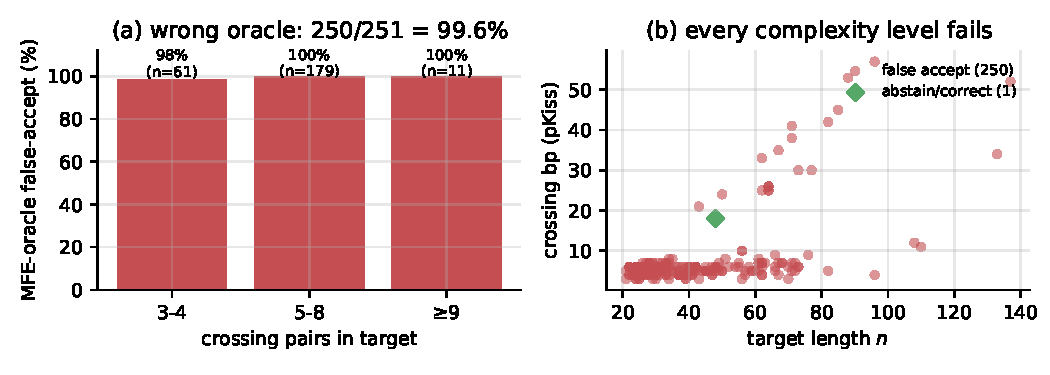
\includegraphics[width=0.95\linewidth]{figs/f_pk.pdf}
\caption{Axis~1, specification projection onto an out-of-domain oracle. (a)~Designs built against the
projected skeleton are accepted by the blind harness for $250/251$ targets, flat across pseudoknot
complexity. (b)~The projection erases the objective at every length and crossing-pair count; the single
non-accept (green) is a target the search could not even skeleton-solve.}\label{fig:pk}
\end{figure}

\begin{table}[t]\centering\small
\begin{tabular}{lcccc}
\toprule
crossing pairs & instances & skeleton-solved & pKiss forms full $T$ & false accepts\\
\midrule
$3$--$4$   & 61  & 60  & 0 & 60\\
$5$--$8$   & 179 & 179 & 0 & 179\\
$\ge 9$    & 11  & 11  & 0 & 11\\
\midrule
\textbf{all} & \textbf{251} & \textbf{250} & \textbf{0} & \textbf{250 ($99.6\%$)}\\
\bottomrule
\end{tabular}
\caption{Specification-projection false accepts by pseudoknot complexity (exact counts, not estimates).
``skeleton-solved'' = design's MFE equals the projected skeleton; ``pKiss forms full $T$'' = pKiss (fixed
config) predicts the full pseudoknot forms.}\label{tab:pk}
\end{table}

\begin{table}[t]\centering\small
\begin{tabular}{lcc}
\toprule
 & pKiss forms $T$ & pKiss does not\\
\midrule
skeleton-solved     & $0$ & $250$\\
not skeleton-solved & $0$ & $1$\\
\bottomrule
\end{tabular}
\caption{Full $2\times2$ contingency over all $251$ instances. The $99.6\%$ is the top-right cell over the
$251$ total; no design that passes the projected check forms the true target.}\label{tab:pkcontingency}
\end{table}

\subsection{Axis 2: the too-weak rung ($92\%$)}\label{sec:axis2}
Now fix the correct oracle and vary only strictness. We take the exact-match ``solutions'' produced by the
cost-optimal search on EteRNA100-V2 ($100$ targets, $5$ seeds, $304$ solved solutions) and re-judge each
under the stronger rungs (Table~\ref{tab:frontier}, Figure~\ref{fig:frontier}a). Acceptance survival
collapses along the ladder: $\match{}\,100\%\to\umfe{}\,91.4\%\to\pfe(0.9)\,8.2\%$. In other words $92\%$
of the sequences that satisfy the cheap ``solved'' criterion are fragile single-structure artifacts that a
robustness verifier rejects; the median target probability is only $\PT{=}0.295$. The set nesting of
Eq.~\eqref{eq:nest} holds with \textbf{zero} violations across all $304$ solutions, confirming the ladder
is genuinely ordered.

\paragraph{The gap is the verifier's, not the solver's.} A natural worry is that this collapse is an
artifact of our replica-exchange solver---perhaps its warm-start biases it toward fragile sequences. It is
not. We repeat the frontier with a \emph{completely independent} solver, ViennaRNA's adaptive-walk
\texttt{RNAinverse} (a different algorithm family, no shared code with REMC), on the targets it can
exact-match ($72$ solutions over $30$ targets, $n\le120$). The collapse reproduces and is if anything
\emph{sharper}: $\match{}\,100\%\to\umfe{}\,83\%\to\pfe(0.9)\,1.4\%$, median $\PT{=}0.15$. Two unrelated
cost-optimal solvers thus emit the same large mass of cheap-verifier-accepted, robustness-failing
solutions, establishing that the over-acceptance is a property of the cheap \emph{verifier}, not of any
particular search.

\paragraph{Not an artifact of the threshold.} The gap is also not an artifact of the specific strong-rung
threshold $\theta{=}0.9$. Sweeping it, survival falls monotonically---$29.9\%$ ($\theta{=}0.5$), $21.1\%$
($0.7$), $8.2\%$ ($0.9$), $1.6\%$ ($0.99$), cluster-bootstrap CIs in Appendix~\ref{app:extended}---so at
\emph{every} robustness bar the large majority of exact-match solutions are rejected; $\theta$ tunes the
size of the gap, not its existence.

\begin{table}[t]\centering\small
\begin{tabular}{lccc}
\toprule
rung & survival & 95\% CI & verify cost\\
\midrule
\match{} (cheap proxy) & $100.0\%$ & $[100.0,100.0]$ & $11.8$\,ms\\
\umfe{}                & $91.4\%$  & $[86.3,96.0]$   & $35.6$\,ms\\
\pfe{}$(0.9)$          & $8.2\%$   & $[2.6,15.6]$    & $52.8$\,ms\\
\bottomrule
\end{tabular}
\caption{RNA acceptance survival across the strictness ladder ($304$ solutions from $100$ targets $\times\,5$
seeds; \emph{cluster} bootstrap $95\%$ CI, resampling targets so within-target seed correlation is
respected). Median $\PT{=}0.295$.}\label{tab:frontier}
\end{table}

The fragility grows sharply with problem hardness (Table~\ref{tab:length}, Figure~\ref{fig:frontier}b):
the exact-match-but-not-robust rate climbs from $71\%$ at $n<50$ to $97$--$100\%$ for $n\ge50$, with mean
\PT{} falling from $0.60$ to $0.27$. (The slight dip at $n\ge200$ reflects that the cheap search can only
reach exact match on the small, GC-rich subset of the longest targets, which happen to be more robust.)
SAT shows the same-direction trend, and we measure it \emph{without any solver} to rule out
solver-selection bias, following the exhaustive-enumeration methodology of \citet{ardelius2008exhaustive}
(Figure~\ref{fig:frontier}c, Table~\ref{tab:sat}). For small formulas ($n=14$) we \emph{enumerate all
$2^{n}$ assignments}, giving exact SAT/UNSAT ($\alpha_c$ is an asymptotic value, so we report the measured
satisfiable fraction, falling $100\%\to57\%$) and the single-flip robustness $\rho$ averaged over the
\emph{entire} solution set of each formula---the true typical robustness, uniform over solutions. The
median-over-solutions $\rho$ falls $0.214\to0.071$ as $\alpha$ rises $3.0\to4.6$ (with a small non-monotone
blip at $4.267$ from few-solution formulas), and the mean solution-set size shrinks $56\to5$. That solution
robustness collapses and solutions cluster/freeze approaching $\alpha_c$ is a \emph{classical} result of the
statistical physics of SAT \citep{krzakala2007clustering,zhou2008frozen,ardelius2008exhaustive}; we claim no
novelty for it, and reuse it only as a decidable strong rung whose collapse \emph{qualitatively mirrors} the
RNA frontier (the two domains share no mechanism, so the shared direction---not any shared number---is the
cross-domain claim).

\begin{table}[t]\centering\small
\begin{tabular}{lccc}
\toprule
length $n$ & solutions & not-robust rate & mean \PT{}\\
\midrule
$<50$        & 63  & $71.4\%$  & $0.60$\\
$50$--$99$   & 71  & $97.2\%$  & $0.43$\\
$100$--$199$ & 112 & $100.0\%$ & $0.27$\\
$\ge 200$    & 58  & $91.4\%$  & $0.31$\\
\bottomrule
\end{tabular}
\caption{Fragility grows with hardness: fraction of exact-match solutions failing \pfe{}, by target
length.}\label{tab:length}
\end{table}

\begin{figure}[t]\centering
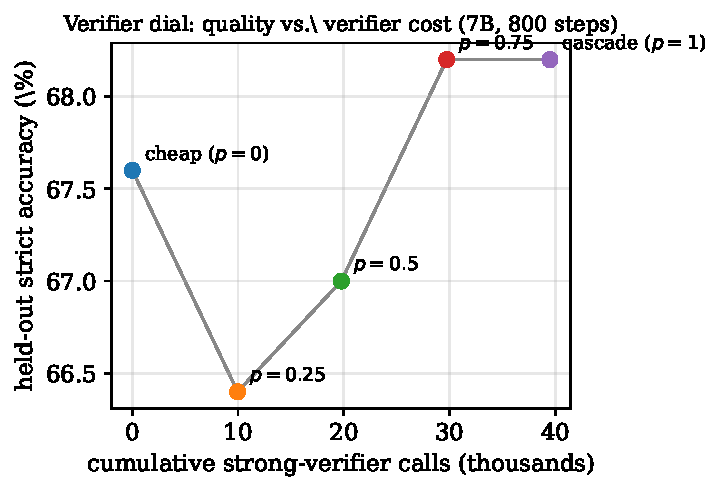
\includegraphics[width=0.98\linewidth]{figs/f1_frontier.pdf}
\caption{The verifier gap (Axis~2). (a)~RNA acceptance survival collapses across the strictness ladder
(error bars: bootstrap $95\%$ CI). (b)~RNA robustness falls with target length. (c)~SAT robustness falls
with clause density toward the 3-SAT threshold. Cheap-proxy solutions are increasingly fragile with
hardness in both domains.}\label{fig:frontier}
\end{figure}

Taken alone, Axis~2 is a criterion mismatch: the sequences genuinely satisfy the cheap predicate, they are
simply not robust. Whether this becomes \emph{reward hacking}---a gap that optimization actively
exploits---requires a controlled optimization experiment, which we supply next.

\section{Optimization-Induced Goodhart, Controlled}\label{sec:goodhart}
To separate a static criterion mismatch from an \emph{optimization-induced} gap, we hold the proposer fixed
(a single Metropolis point-mutation kernel and schedule) and vary \emph{only} the reward predicate: a
\emph{cheap} objective (exact match, then a continuous MFE-stability term that does not saturate) versus a
\emph{strong} objective (ensemble defect, which rewards robustness directly). Two notes on the design.
First, the gold judge ($\PT\ge0.9$) is \emph{not} the strong optimization signal (ensemble defect): the two
are related robustness measures but not identical, so the strong arm is judged on a metric it does not
directly optimize---a deliberately \emph{conservative} test. Second, because the proposer, the search, and
the budget are identical across arms, any difference is attributable to the reward---i.e.\ to the
verifier---and to nothing else, and no reinforcement learning is required: a classical optimizer suffices
and avoids the confounds of RL dynamics. The study uses $18$ targets ($n\le50$) $\times\,5$ seeds
$=90$ (seed, target) units per cell.

The Goodhart signature is the \emph{divergence between the proxy and the true objective within the cheap
arm} (Table~\ref{tab:goodhart}, Figure~\ref{fig:goodhart}). As budget grows, the cheap arm optimizes its
own objective successfully---its exact-match rate climbs monotonically $31\%\to51\%\to60\%\to70\%$---yet
its robustness does \emph{not} follow: it peaks at $26.7\%$ (budget $1{,}000$) and then \emph{declines} to
$15.6\%$. Proxy up, true objective flat-then-down: this is precisely reward hacking, not a static
mismatch. The strong arm is the control: there proxy and robustness rise \emph{together}
($23\%\to50\%$ exact-match, $12.2\%\to33.3\%$ robust). At the largest budget the two arms' robustness
differs by $17.7$ points with \emph{disjoint} $95\%$ confidence intervals ($[8.9,23.3]$ vs.\ $[24.4,43.3]$).
Harder optimization of the cheap proxy buys \emph{more of the proxy and less robustness}; only optimizing
the true objective buys robustness. This gives the deterministic, dial-able instrument the LLM-side
literature \citep{gamingverifiers} approximates with noisy judges: here the effect is exactly attributable
rather than entangled with policy-optimization dynamics.

\begin{table}[t]\centering\small
\begin{tabular}{lccc}
\toprule
budget & \multicolumn{2}{c}{cheap-reward arm} & strong-reward arm\\
(evals) & exact-match (proxy) & robust $\PT{\ge}0.9$ & robust $\PT{\ge}0.9$\\
\midrule
$200$     & $31.1\%$ & $17.8\%$ $[10,26]$ & $12.2\%$ $[6,19]$\\
$1{,}000$ & $51.1\%$ & $26.7\%$ $[18,37]$ & $18.9\%$ $[11,28]$\\
$5{,}000$ & $60.0\%$ & $20.0\%$ $[12,29]$ & $28.9\%$ $[20,39]$\\
$20{,}000$& $\mathbf{70.0\%}$ & $\mathbf{15.6\%}$ $[9,23]$ & $\mathbf{33.3\%}$ $[24,43]$\\
\bottomrule
\end{tabular}
\caption{Controlled Goodhart (RNA, $18$ targets $\times\,5$ seeds $=90$ units/cell; bootstrap $95\%$ CI).
In the cheap arm the \emph{proxy} (exact-match) rises to $70\%$ while its \emph{robustness} peaks then
falls to $15.6\%$---the proxy--objective divergence that defines Goodhart. The strong arm (control) improves
both. Raw numerators are $\text{rate}\times90$.}\label{tab:goodhart}
\end{table}

\begin{figure}[t]\centering
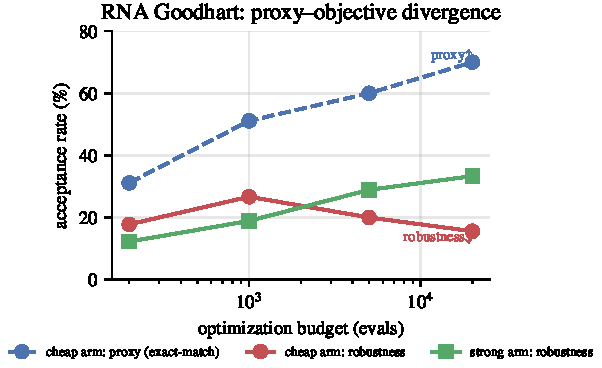
\includegraphics[width=0.6\linewidth]{figs/f2_goodhart.pdf}
\caption{Controlled Goodhart (RNA, fixed proposer, $18$ targets $\times\,5$ seeds). Within the cheap arm,
the \emph{proxy} it optimizes (exact-match, dashed) rises to $70\%$ while its \emph{robustness} (red) peaks
then falls---the proxy--objective divergence that defines reward hacking. The strong-arm control (green)
improves robustness monotonically.}\label{fig:goodhart}
\end{figure}

\paragraph{Domain dependence (an honest boundary).} The same construction in SAT produces only a mild gap:
both arms hold $V_0=100\%$, and the strong arm's median $\rho$ rises only $0.100\to0.117$ while the cheap
arm's stays flat; neither clears the robust threshold. Goodhart severity is therefore
\emph{domain-dependent}---pronounced where the cheap objective admits many competing near-optimal
structures (RNA), mild where satisfying assignments are structurally uniform (SAT). We report this rather
than suppress it: the cross-domain generality of the paper rests on the frontier and cost mirrors
(\S\ref{sec:gap},\ref{sec:cost}), which hold in both domains, with the Goodhart leg carried by RNA. A
further honesty: the \emph{existence} of the effect is what our controlled design establishes; its
\emph{magnitude} depends on how misaligned the cheap proxy is with the robustness objective, which is a
design choice we do not calibrate. We chose a continuous but robustness-agnostic cheap objective; a cheap
proxy engineered to correlate with robustness would show a smaller gap. The claim is therefore that a
robustness-agnostic cheap reward \emph{can} be optimized while robustness stalls, not that any cheap reward
must produce a gap of this size.

\section{Cross-Domain Validation on an LLM Code Verifier}\label{sec:llm}
RNA and SAT are deterministic proxies chosen for control; the domain the paper is \emph{about} is LLM
verification. We therefore test whether the mechanisms reproduce on a real LLM code verifier---the
canonical RLVR setting---and, crucially, whether the paper's \emph{dial-ability} claim (tightening the
rung reduces over-acceptance) holds there. We use $19$ small Python function-writing problems; each carries
an ordered test pool whose first entries are ``happy-path'' assertions and whose remainder are edge cases.
The cheap rung of strictness~$k$ accepts a program that passes the first $k$ tests; the strong rung
requires all tests---so the rungs are nested by construction and $k$ \emph{dials} the cheap verifier from
weak ($k{=}1$) to stronger ($k{=}3$). Four fixed proposers spanning capability
(\texttt{gpt-3.5-turbo}, \texttt{llama-3.1-8b}, \texttt{qwen-2.5-coder-32b}, \texttt{gpt-4o-mini}, all at
temperature $0.8$) sample $12$ candidates per problem, executed in a sandbox; best-of-$N$ selection is the
optimization budget, the cheap arm selecting blind to held-out (as a reward-hacking policy must).

\paragraph{Axis-2 transfers, across models.} At the weak rung ($k{=}1$), $7.5$--$9.2\%$ of the programs
that pass the provided tests fail the held-out population in three of four models (Table~\ref{tab:llm}); the
mechanism is exactly ``the cheap rung is satisfiable without the property one wants'' (e.g.\ floor division
passing $\lfloor 7/2\rfloor{=}3$ while truncating $\lfloor -7/2\rfloor$; banker's rounding). The gaps are
smaller than RNA's $92\%$---capable models get most edge cases right---but nonzero, deterministic, and
model-general. (The code-specialized \texttt{qwen} passes the provided tests far less often, $138/228$, and
when it does it is always robust---a different, honest failure mode.)

\paragraph{Dial-ability transfers (the key result).} Strengthening the cheap rung from $k{=}1$ to $k{=}3$
\emph{monotonically reduces} the false-accept mass in \emph{every} model that had any: $7.5\%\to5.4\%$
(\texttt{gpt-3.5}), $9.2\%\to1.0\%$ (\texttt{llama}), $7.5\%\to0.0\%$ (\texttt{gpt-4o-mini})
(Figure~\ref{fig:llm}a). This is the paper's central ``dial the rung, dial the over-acceptance'' claim,
demonstrated on a real LLM verifier: a practitioner \emph{can} trade a little more test-writing for a
measurable reduction in gamed acceptances.

\paragraph{Goodhart transfers, model-dependently.} Under best-of-$N$, the strong arm's robustness climbs
above the cheap arm's for \texttt{llama} ($89.5\%\to100\%$, Figure~\ref{fig:llm}b) and \texttt{gpt-4o-mini}
($89.5\%\to94.7\%$), while for \texttt{gpt-3.5} and \texttt{qwen} the two arms coincide. As in RNA vs.\ SAT,
the Goodhart-under-selection effect is real but domain/model-dependent; the robust cross-model findings are
the Axis-2 gap and its dial-ability.

\paragraph{Scope.} Magnitudes are modest---capable models on tractable problems---so we claim transfer of
\emph{direction, mechanism, and dial-ability}, not that LLM verifier gaps match RNA's. The value is that the
paper's prescriptions are here \emph{measured on the target domain}, not argued by analogy.

\begin{figure}[t]\centering
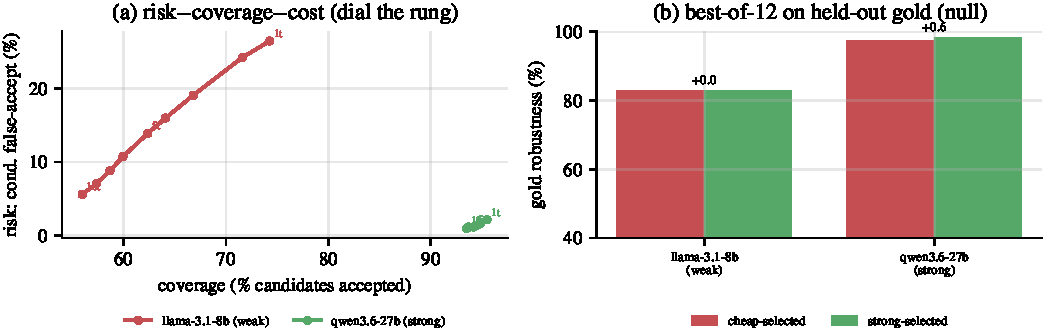
\includegraphics[width=\linewidth]{figs/f_llm.pdf}
\caption{LLM code verifier (4 models, $19$ problems). (a)~Dial-ability: strengthening the cheap rung
($k{=}1\to3$) monotonically cuts false-accept mass in every model that had any. (b)~Goodhart under
best-of-$N$ on \texttt{llama-3.1-8b}: the cheap proxy is pinned high while its robustness is flat and the
strong arm's climbs---the same divergence as RNA.}\label{fig:llm}
\end{figure}

\begin{table}[t]\centering\small
\begin{tabular}{lcccc}
\toprule
model & FP-mass $k{=}1$ & FP-mass $k{=}3$ & \multicolumn{2}{c}{best-of-12 robust}\\
      &                 &                 & cheap & strong\\
\midrule
\texttt{gpt-3.5-turbo}   & $7.5\%$ & $5.4\%$ & $94.7$ & $94.7$\\
\texttt{llama-3.1-8b}    & $9.2\%$ & $1.0\%$ & $89.5$ & $\mathbf{100.0}$\\
\texttt{qwen-coder-32b}  & $0.0\%$ & $0.0\%$ & $63.2$ & $63.2$\\
\texttt{gpt-4o-mini}     & $7.5\%$ & $0.0\%$ & $89.5$ & $94.7$\\
\bottomrule
\end{tabular}
\caption{LLM code verifier over-acceptance ($19$ problems, $12$ samples). False-accept mass falls as the
cheap rung is dialed stronger ($k{=}1\to3$) in every engaging model; best-of-$12$ shows the Goodhart gap
where it appears.}\label{tab:llm}
\end{table}

\section{The Cost of Verification}\label{sec:cost}
If stronger verifiers were always vastly more expensive, the tension would be a simple budget line. They
are not, and the true cost structure is more interesting. Figure~\ref{fig:cost} and Table~\ref{tab:cost}
give end-to-end verification costs. The headline is that \emph{the cost of strictness depends on whether
the strong predicate reuses the cheap oracle's computation or must probe a neighborhood}. On RNA the three
strictness rungs all scale as $\sim n^{2.8}$ (i.e.\ $O(n^3)$, the folding complexity) and lie within a
$\sim4\times$ constant factor ($98/301/384$\,ms at $n=300$), because \umfe{} and \pfe{} are one extra
$O(n^3)$ partition-function pass over the same DP tables the MFE already builds. In SAT the within-domain
ladder is far steeper---$V_0$ is $O(m)$, $\rho$ is $O(nm)$, the radius-$2$ ball is $O(n^2m)$, spanning
$\sim400\times$ at $n=200$---because certifying robustness there requires an explicit Hamming-ball scan
with no reuse. So ``stronger'' is cheap when the strong rung amortizes the cheap oracle's work and expensive
when it does not; this, not a blanket ``stronger costs more,'' is the cost structure a designer should plan
around. We state this as a \emph{contrast consistent with computation reuse across our two domains}
($n=2$), not as an established general principle---establishing it as a law would need strong rungs of both
reuse and no-reuse type within a single domain. We deliberately do \emph{not} draw a conclusion about the
cost of \emph{switching oracles}: our
pseudoknot branch (pKiss) is measured only at $n=30$--$150$ and is startup-dominated ($\sim121$\,ms, flat),
so it is \emph{not length-matched} to the RNA strictness rungs (reported to $n=300$) and---at the lengths
we can compare---is not more expensive than \pfe{}. A length-matched cross-oracle cost comparison is left
to future work; Table~\ref{tab:cost} reports the branch cost only as a range, not as a claim.

\begin{figure}[t]\centering
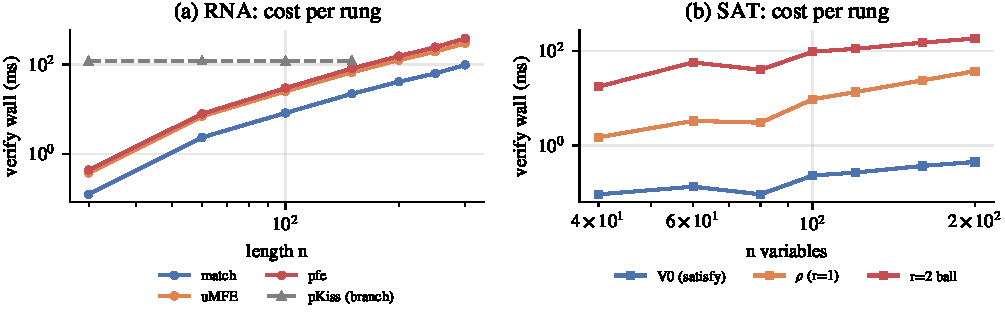
\includegraphics[width=0.98\linewidth]{figs/f3_cost.pdf}
\caption{Verification cost per rung. (a)~RNA: strictness rungs are $\sim O(n^3)$ within $\sim4\times$;
pKiss (branch) is startup-dominated. (b)~SAT: the within-domain robustness ladder is steeper.}\label{fig:cost}
\end{figure}

\begin{table}[t]\centering\small
\begin{tabular}{lccl}
\toprule
rung & scaling & cost@max\,$n$ & note\\
\midrule
RNA match & $n^{2.78}$ & $98$\,ms & cheap proxy ($n{=}300$)\\
RNA uMFE  & $n^{2.79}$ & $301$\,ms & $\sim3\times$ match\\
RNA pfe   & $n^{2.84}$ & $384$\,ms & $\sim4\times$ match\\
RNA pKiss & --- & $\sim121$\,ms & branch (startup, flat)\\
SAT $V_0$ & $O(m)$ & $0.45$\,ms & cheap proxy ($n{=}200$)\\
SAT $\rho$ & $O(nm)$ & $38$\,ms & $\sim83\times$\\
SAT $r{=}2$ & $O(n^2 m)$ & $185$\,ms & $\sim410\times$\\
\bottomrule
\end{tabular}
\caption{End-to-end verification cost. Strictness within RNA is a small constant factor (shared
partition-function pass); in SAT it is steep (Hamming-ball scan). The pKiss branch is reported only as a
range at $n\le150$ and is \emph{not} length-matched to the RNA rungs---no cross-oracle cost claim is drawn
from it.}\label{tab:cost}
\end{table}

\section{Sound and Risk-Calibrated Routing}\label{sec:routing}
Given a stream of candidates and a designated \emph{gold} rung (here \pfe{}), a practitioner wants the gold
verdict at the lowest possible cost. The ladder structure makes two policies analyzable exactly.

\subsection{A sound cascade}
\begin{theorem}[Sound cascade, $\epsilon=0$]\label{thm:cascade}
Under the nesting of Eq.~\eqref{eq:nest}, the cheapest-first cascade---evaluate rungs in cost order,
reject at the first rung that rejects, and escalate a candidate to gold only if it passes every cheaper
rung---produces \emph{exactly} the gold verdict on every input, and pays the gold cost only on candidates
that pass all cheaper rungs.
\end{theorem}
The result is elementary---it is short-circuit evaluation under set nesting---and we present it as a
\emph{correctness guarantee for the instrument}, not as a deep theorem: its value is that it licenses the
cost savings below without ever risking a wrong verdict. The proof (Appendix~\ref{app:proofs}) is immediate
from nesting: a cheap-rung reject is a certain gold reject, so early rejection is always sound, and accepts
are escalated to gold, so accepts are always correct. Measured on our workloads, the cascade is
exact---correctness $100\%$ with \textbf{zero} unsound cases on both. Its \emph{saving}, however, is
workload-dependent (Table~\ref{tab:routing}): on a reject-heavy workload ($12$ random candidates per
target, $1$ solution) it saves $+62.5\%$ versus always-running-gold ($0.53$ vs.\ $1.42$\,ms per candidate),
because the cheap rungs filter out non-solutions before the expensive check; on an accept-heavy one ($0$
random, $6$ solutions per target) it \emph{costs} $-19.2\%$ ($1.44$ vs.\ $1.21$\,ms), because nothing is
cheaply rejected and the cheap rungs are pure overhead. The cascade is thus a \emph{reject filter}:
valuable on failure-heavy streams---such as early RL training, where most rollouts are wrong---and a net
cost on streams where most candidates are genuine.

\begin{table}[t]\centering\small
\begin{tabular}{lcccc}
\toprule
workload & correctness & unsound & E[cost] vs gold & cascade saving\\
\midrule
reject-heavy & $100\%$ & $0$ & $0.53$ / $1.42$\,ms & $+62.5\%$\\
accept-heavy & $100\%$ & $0$ & $1.44$ / $1.21$\,ms & $-19.2\%$\\
\bottomrule
\end{tabular}
\caption{Sound cascade (Theorem~\ref{thm:cascade}), $15$ targets ($n\le65$). Always exact; its saving is a
reject-filter---positive only when the workload contains cheaply-rejectable candidates (reject-heavy:
$12$ random $+1$ solution per target; accept-heavy: $6$ solutions, no random).}\label{tab:routing}
\end{table}

\subsection{Risk-calibrated stopping}
To save more, one may \emph{stop and accept} at a cheaper rung, trading correctness for cost and incurring
a false positive whenever the gold rung would have rejected. We calibrate on a held-out split: choose the
cheapest rung whose false-positive rate has a Clopper--Pearson \emph{upper} confidence bound $\le\epsilon$
at confidence $1-\delta$, then apply it to a test split. To make costs comparable across workloads of
different length composition, we report expected cost as a \emph{fraction of the always-gold cost}
(Figure~\ref{fig:routing}); on the reject-heavy workload the sound cascade already sits at $0.375\times$
always-gold, its saving coming entirely from cheap \emph{rejects}. The question is whether cheap
\emph{accepts} can lower it further. They cannot: the \match{} rung accepts $5.1\%$ of candidates while the
gold rung accepts $0.0\%$, so essentially every match-accept is a false positive (match-rung
$\mathrm{FP}\approx100\%$). No rung cheaper than gold therefore has a Clopper--Pearson upper bound below any
tolerance $\epsilon\le0.9$, and the calibrated frontier stays pinned at gold ($0.39\times$ always-gold) for
every such $\epsilon$. We are precise about the scope of this statement: it is an \emph{empirical,
workload-specific} incompressibility, not a theorem. It holds for this candidate distribution, cheap rung,
gold threshold, confidence level, and calibration split; a different proposer or training stage would give
a different false-positive rate. What is robust is the mechanism---once a cheap rung is highly gameable,
there is no admissible cheaper-than-gold accept rule---and this is exactly the regime optimization pressure
produces (\S\ref{sec:goodhart}).

\begin{figure}[t]\centering
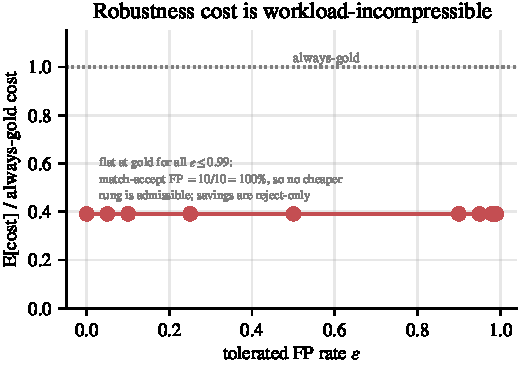
\includegraphics[width=0.62\linewidth]{figs/f_routing.pdf}
\caption{Risk-calibrated routing (costs as a fraction of always-gold, so workload length-composition
cancels). Even tolerating up to $\epsilon=0.9$ false positives, the calibrated rule cannot drop below the
sound-cascade cost: cheap-accept has $98\%$ FP (upper bound $\approx0.999$), so savings come only from
cheap rejects, not cheap accepts. Empirical and workload-specific, not a general theorem.}\label{fig:routing}
\end{figure}

\section{Discussion: Implications for Reward Design}\label{sec:discussion}
The results compose into a few concrete recommendations for anyone building a verifiable reward.

\paragraph{Model the verifier as a graph, and abstain out of domain.} Axis~1 shows that the most dangerous
failure is not a slightly-too-lenient threshold but an oracle that cannot represent the objective at all,
which then certifies nearly everything. The remedy is architectural: attach a domain-of-validity gate that
abstains rather than scoring a projected version of the task. In RLVR terms, a reward model should return
``I cannot judge this'' as a first-class output, and the training loop should treat abstention differently
from a low score.

\paragraph{Exact-match is not robustness, and it saturates.} Axis~2 shows that a binary exact-match reward,
even when perfectly faithful in the sense of being correctly computed, is a weak proxy for a robustness
objective, and that the gap widens with problem hardness. A continuous, non-saturating proxy (here, target
Boltzmann probability or ensemble defect) is what lets optimization actually build robustness
(\S\ref{sec:goodhart}). Reward designers should prefer continuous robustness-aware signals over binary
pass/fail wherever the true objective has a robustness component.

\paragraph{Cheap-first cascades are reject filters, not free lunches.} The sound cascade
(Theorem~\ref{thm:cascade}) is exactly correct and can save substantially---but only on failure-heavy
streams. Its value is highest early in training (most rollouts wrong) and erodes as the policy improves.
A practitioner should expect its benefit to be a moving target over a training run, not a fixed speedup.

\paragraph{Budget for robustness certification; it will not compress.} The risk-calibrated analysis says
that when the cheap rungs are highly gameable---the common case under optimization pressure---there is no
cheap surrogate for the strong verifier at acceptable risk. The strong rung must be run. The good news from
\S\ref{sec:cost} is that, at least in RNA, strictness itself is cheap; the budget goes to running the right
oracle, not to a steep strictness ladder.

\paragraph{Instantiating the ladder for LLM verifiers.} The construction transfers to the domains where
RLVR is actually deployed. For \emph{code}, the analogue of \match{} is ``passes the provided unit tests'';
\umfe{} is ``passes tests and no near-duplicate program of equal length passes a superset'' (the
degenerate-solution loophole, e.g.\ reward-hacked stubs); \pfe{} is ``passes a held-out, mutation-generated
test population with margin''---a robustness rung whose threshold is the dial. For \emph{math}, \match{} is
``final answer matches''; the strong rung is ``the proof survives a checker over paraphrased/perturbed
statements.'' For \emph{pseudoknots read as out-of-domain tasks}, the code analogue of Axis~1 is grading a
concurrency bug with a single-threaded test harness: the oracle structurally cannot see the failure and
certifies it as fixed. Our results then predict, and prescribe: (i) attach a domain-of-validity gate, since
a blind oracle false-accepts almost everything; (ii) prefer a continuous held-out-population score to a
binary pass, since binary saturates and does not build robustness under optimization; and (iii) budget for
the strong rung, since no cheap surrogate is safe once the policy games the cheap one. The value of the
deterministic testbed is that these prescriptions are \emph{measured}, not assumed.

\section{Related Work}\label{sec:related}
\paragraph{The verifier problem in RLVR.} A growing literature documents that verifiers get gamed: the
trilemma of scalability, faithfulness, and robustness \citep{verificationhorizon}; extensional versus
intensional gaming \citep{gamingverifiers}; deterministic reward-hacking measurement at scale
\citep{hackverifiable}; rubric hacking \citep{rubricrewardhacking}; and robust optimization against
correlated proxies \citep{correlatedproxies,hiddencosts}. A parallel line builds \emph{benchmarks} for
reward hacking---embedding detectable exploits in environments and measuring whether agents take them
\citep{hackverifiable,rewardhackbench}, or fuzzing RLVR verifiers to find bugs before a policy learns them
\citep{fuzzverifiers}. Two things distinguish our work from both lines. First, \emph{target}: they study
verifiers that are noisy (learned judges, rubrics) or deliberately hackable (embedded bugs), and ask
whether they are exploited; we study verifiers that are \emph{fully decidable and correct} and show they
still over-accept---so the failure is not a bug to be fuzzed out but a \emph{misspecification} (wrong
oracle, weak rung) intrinsic to the choice of predicate. This sharpens the community's implicit assumption
that a deterministic verifier is safe. Second, \emph{apparatus}: rather than a single environment, we give
a \emph{strictly nested, dial-able, priced} family of predicates on one problem, so the acceptance gap is
quantified with zero evaluator variance, the Goodhart effect is attributed to the verifier alone, routing
is \emph{proved} sound, and the cost of robustness is finite-sample-calibrated---none of which a single
hackable environment supports.

\paragraph{RNA design and SAT solution geometry.} RNA robustness objectives---ensemble defect, unique MFE,
target probability---are standard design targets \citep{zadeh2011nupack,zhou2023samfeo,ribopo}, and the
RNAfold/pKiss split for pseudoknots is well established \citep{rnainvbench,janssen2015pkiss}; we claim none
of these, but treat the \emph{ladder} over them as the object of study. Likewise, SAT solution robustness
(clustering, frozen variables, and its exhaustive-enumeration measurement) is classical statistical physics
\citep{krzakala2007clustering,zhou2008frozen,ardelius2008exhaustive}; we reuse both the phenomenon and the
enumeration method, and add only the framing of $\rho$ as a decidable strong rung mirroring RNA.

\paragraph{Companion family.} This is the verifier-economics member of a companion family of self-improvement
studies. It adopts the four-coordinate diagnostic of \citet{determinismmanifold} and the actuation
coordinate of \citet{actuation} (cited, not re-derived), and \emph{refines} the oracle-residue thesis of
\citet{oracleresidue}: their clean-oracle pole holds \emph{when the verifier is correctly selected}; we make
verifier selection a variable and show a cost-optimal search is pulled toward the gameable rung. Unlike the
compounding adjudication of \citet{compoundingprofile}, which pins correctness ungameable to isolate
compounding, we \emph{dial} verifier strength to study the gaming--cost tradeoff---opposite moves on the
same axis---and we sharpen the family's notion of ``exact'': a decidable, correctness-ungameable verifier
can still be a weak proxy for a \emph{robustness} objective. Unlike \citet{greenzone}, whose learning result
is null on capability, our routing result concerns \emph{cost} at fixed correctness (the solve set is never
changed).

\section{Limitations}\label{sec:limits}
We state the scope conditions plainly. \textbf{(i)~Model-relative verdicts.} ``Solved'' means solved under
the declared folding/energy model, never biophysical truth; this is the regime every deployed verifier
already operates in, but it is a modeling choice, not ground truth. \textbf{(ii)~Classical optimization,
not RL.} The Goodhart demonstration (\S\ref{sec:goodhart}) uses a fixed classical proposer, which isolates
the verifier's contribution cleanly but does not reproduce RL-specific dynamics; we position it as a
measurement instrument, not an RL result. \textbf{(iii)~Domain-dependent Goodhart.} The Goodhart effect is
strong in RNA and mild in SAT; the cross-domain claims rest on the frontier and cost mirrors, not on
Goodhart. \textbf{(iv)~One robustness notion.} $\rho$ (single-flip) and \pfe{} (Boltzmann probability) are
particular robustness measures; solution-cluster / backbone membership is a richer, costlier strong rung we
do not evaluate here. \textbf{(v)~Survivor bias.} The Axis-2 frontier is computed only over targets the
cost-optimal search can exact-match; harder targets that never reach \match{} are absent from every length
bin, not only $n\ge200$. This biases the analyzed set toward the easier, and if anything \emph{more}
robust, sequences, so the true over-acceptance is likely \emph{under}-stated; the second-solver control
(\S\ref{sec:axis2}) shows the collapse is not specific to which subset one solver reaches, but a design
that enumerates or exhaustively solves small targets would remove the bias entirely. \textbf{(vi)~Scale.}
The study is moderate-scale ($251$ pseudoknots; $100$ RNA targets $\times$ $5$ seeds; $18$-target Goodhart;
$8$ SAT densities $\times$ $40$ enumerated instances), with cluster-bootstrap and finite-sample intervals
throughout; larger sweeps would sharpen the intervals but are not expected to change the direction of any
reported effect.

\section{Future Work}\label{sec:future}
Three extensions follow directly. First, \emph{richer robustness rungs}: replacing single-flip $\rho$ and
Boltzmann probability with cluster-membership or free-energy-gap predicates would extend the ladder upward
and test whether the near-incompressibility of \S\ref{sec:routing} strengthens. Second, \emph{a third
deterministic domain} (e.g.\ program synthesis against a formal specification, or constraint-satisfaction
scheduling) would turn the cross-domain claim from two points into a trend. Third, \emph{closing the loop
to RL}: using the dial-able ladder as the reward in an actual policy-optimization run would test whether
the controlled Goodhart effect measured here reproduces under learned proposers, and whether the
sound-cascade reject-filter delivers its predicted early-training speedup in practice.

\section{Conclusion}\label{sec:conclusion}
``Solved'' is a choice of verifier, not a fact. In two deterministic domains we made that choice a
dial-able, priced, decidable ladder; measured how much a cost-optimal search over-accepts along two
independent axes and how this worsens with hardness; showed the gap is optimization-induced through a
controlled, RL-free experiment; priced the ladder honestly, separating cheap strictness from expensive
oracle choice; and proved a sound routing cascade whose risk-calibrated relaxation reveals robustness
certification to be near-incompressible. The contribution is the instrument, not a new phenomenon: a place
to measure the verifier problem exactly, in domains where the truth value is computed rather than judged.

\section*{Reproducibility Statement}
Every reported number is produced by a deterministic run under a fixed, reported seed, against a pinned
computational model (ViennaRNA~2.7.2 / Turner~2004 / $37^\circ$C / \texttt{dangles=2} for RNA; exact CNF
evaluation for SAT). The two acceptance-set claims are proved in full (Appendix~\ref{app:proofs}); the
solver, cost model, and statistical procedure are specified in Appendix~\ref{app:methods}; per-density and
per-length breakdowns are in Appendix~\ref{app:extended}; and known implementation caveats (a bounded
wall-budget overshoot on very large targets; the ViennaRNA version-pinning needed for leaderboard
comparison) are disclosed in Appendix~\ref{app:repro}. The harness, all experiment scripts, and the
per-instance JSON behind every figure and table are released so that each result can be regenerated
end-to-end.

\appendix
\section{Proofs}\label{app:proofs}
\begin{proposition}[Nesting]\label{prop:nest}
For $\theta>\tfrac12$, $\pfe(\theta)\subseteq\umfe\subseteq\match$. The bound $\theta>\tfrac12$ is tight.
\end{proposition}
\begin{proof}
$\umfe\subseteq\match$ is immediate: if $T$ is the unique minimum-free-energy structure of $x$, then in
particular $\mathrm{MFE}(x)=T$, so $x\in\match$. For $\pfe(\theta)\subseteq\umfe$ with $\theta>\tfrac12$,
suppose $\PT{\mid}x\ge\theta>\tfrac12$. The Boltzmann distribution assigns each secondary structure $S$ a
weight $p(S)=e^{-E(S)/RT}/Z\ge0$ with $\sum_S p(S)=1$, and $p(S)$ is strictly decreasing in $E(S)$. If some
$S'\ne T$ had $E(S')\le E(T)$, then $p(S')\ge p(T)=\PT{\mid}x\ge\theta>\tfrac12$, whence
$p(S')+p(T)>1$, contradicting $\sum_S p(S)=1$. Hence $E(S)>E(T)$ for every $S\ne T$: $T$ is the strict
unique MFE and $x\in\umfe$. Tightness: at $\theta=\tfrac12$, take a sequence with two structures of exactly
equal minimum energy (and all others strictly higher); it has $\Pr[T]=\tfrac12\ge\theta$ but a degenerate
MFE, so $x\in\pfe(\tfrac12)\setminus\umfe$. Such degeneracy is realizable in the declared model: the
Turner-2004 energy function is a finite sum of table entries, so distinct structures can carry numerically
equal energies (a symmetric hairpin pair being the simplest witness), and ViennaRNA's co-optimal
enumeration reports exactly these ties. More generally, for any $\theta\le\tfrac12$ one can place two
minimum-energy structures at weights $\theta$ and $1-\theta$, again realizing $\pfe(\theta)\setminus\umfe$;
hence no threshold $\theta\le\tfrac12$ yields the inclusion, and $\theta>\tfrac12$ is exactly the
admissible range.
\end{proof}

\begin{proof}[Proof of Theorem~\ref{thm:cascade}]
Order the rungs by cost as $R_1\supseteq R_2\supseteq\dots\supseteq R_g$, where the inclusions hold by
Eq.~\eqref{eq:nest} and $R_g$ is the gold rung. The cascade evaluates $R_1,R_2,\dots$ in order; it rejects
at the first $R_i$ with $x\notin R_i$, and it accepts (labeling the candidate gold-accepted) only if
$x\in R_i$ for all $i\le g$. \emph{Soundness of rejection:} if the cascade rejects at $R_i$, then
$x\notin R_i$; since $R_i\supseteq R_g$, also $x\notin R_g$, a true gold reject. \emph{Soundness of
acceptance:} if the cascade accepts, then in particular $x\in R_g$, a true gold accept. Thus the cascade
output equals the gold verdict on every $x$. The gold rung $R_g$ is evaluated only on inputs that passed
every cheaper rung $R_i$, $i<g$; all others are decided by a strictly cheaper rung.
\end{proof}

\section{Methods}\label{app:methods}
\paragraph{Solver (RNA).} The cost-optimal search is replica-exchange Monte Carlo. Eight replicas run on a
geometric temperature ladder over $[0.15,4.0]$. Each epoch, every replica performs a chunk of $300$
Metropolis moves (single-base and paired-base mutations, the latter respecting the target pair table), then
adjacent replicas attempt a parallel-tempering swap with the standard Metropolis criterion. A structural
warm-start seeds all replicas with a GC-stiff assembly consistent with the target. A no-progress guard stops
the search after $8$ epochs without global improvement. A defect-cluster \emph{endgame} performs last-mile
repair on near-misses (base-pair distance $\le6$): it identifies the unformed target pairs, their competing
``intruder'' pairs, and flanking positions, and jointly reassigns them---a coordinated multi-base move that
single-position search cannot reach---optimizing lexicographically over (base-pair distance, ensemble
defect). The whole search, endgame included, is bounded by a shared budget (maximum oracle calls and wall
time), so verification and search costs are both accounted. SAT candidates come from a WalkSAT-style noisy
local search.

\paragraph{Verifier implementation.} \match{} tests string equality of $\mathrm{MFE}(x)$ with $T$.
\umfe{} does not rely on the folding routine's choice of a single MFE representative: we enumerate the set
of \emph{co-optimal} structures with ViennaRNA's suboptimal-folding routine at a narrow energy window
(default $\delta=0.01$\,kcal/mol above the MFE) and count how many lie at the MFE energy within a
$10^{-6}$\,kcal/mol tolerance; $x\in\umfe$ iff that count is exactly one and it equals $T$. The narrow
window is both correct (structures above the MFE energy are discarded by the tolerance filter) and
bounded, avoiding the exponential blow-up of enumerating a wide suboptimal band. \pfe{} computes the
partition function once and reads off $\PT{\mid}x=\Pr[T]$; degeneracy and floating tie-breaking are handled
by the same energy tolerance. All three reuse the fold\_compound built for \match{}.

\paragraph{Cost model.} Verification cost is the wall-clock time from the raw pair $(x,T)$ to a Boolean
verdict, measured in-process with warm folding caches and reported as the median over repetitions ($15$ for
RNA, $25$ for SAT). ``Warm cache'' means the ViennaRNA model parameters are loaded once per process; each
timed call still builds its own DP tables, so the numbers are per-verdict, not amortized across a batch.
Scaling exponents are least-squares fits of $\log(\text{cost})$ against $\log n$. The currency generalizes
additively to solver CPU-seconds and, for an LLM verifier, to tokens.

\paragraph{Statistics.} Rates carry \emph{cluster} bootstrap $95\%$ confidence intervals ($B=5000$),
resampling whole \emph{targets} (with all of their seeds) rather than individual seed$\times$target rows,
so that the non-independence of seeds within a target is respected; this widens the intervals relative to
a naive row bootstrap (e.g.\ \pfe{} survival $[5.3,11.5]\to[2.6,15.6]$) and we report the wider, correct
ones. False-positive rates carry one-sided Clopper--Pearson upper bounds at confidence $1-\delta$,
$\delta=0.05$. The nesting check counts, per solution, any ordered rung pair violating Eq.~\eqref{eq:nest};
we observed none.

\section{Extended Results}\label{app:extended}
Table~\ref{tab:sat} gives the \emph{exhaustive} SAT frontier: for each of $40$ random formulas per density
at $n=14$ we enumerate all $2^{14}$ assignments, so satisfiability is exact and $\rho$ is averaged over the
\emph{entire} solution set of each formula (uniform over solutions, no solver). This removes the
solver-selection bias that would afflict computing $\rho$ on a single WalkSAT-found assignment. Both the
satisfiable fraction and the median-over-solutions robustness fall as density rises, and the solution set
shrinks by an order of magnitude; the trend is the same direction as RNA, though (unlike a mechanism-shared
replica) not numerically identical and with a small non-monotone point at $\alpha_c$ driven by
few-solution formulas.

\begin{table}[t]\centering\small
\begin{tabular}{lccc}
\toprule
$\alpha$ & satisfiable & median $\rho$ over all solutions & mean $|$solutions$|$\\
\midrule
$3.0$   & $100.0\%$ & $0.214$ & $56.3$\\
$3.4$   & $97.5\%$  & $0.214$ & $29.8$\\
$3.8$   & $90.0\%$  & $0.143$ & $17.6$\\
$4.0$   & $87.5\%$  & $0.143$ & $13.4$\\
$4.2$   & $77.5\%$  & $0.107$ & $9.2$\\
$4.267$ & $67.5\%$  & $0.143$ & $10.2$\\
$4.4$   & $62.5\%$  & $0.071$ & $6.4$\\
$4.6$   & $57.5\%$  & $0.071$ & $4.9$\\
\bottomrule
\end{tabular}
\caption{Exhaustive SAT frontier ($n=14$, all $2^{14}$ assignments enumerated, $40$ formulas per density).
Satisfiability is exact; $\rho$ is the median over a formula's \emph{entire} solution set. Robustness and
solution-set size both fall toward and past the (asymptotic) 3-SAT threshold $\alpha_c\approx4.267$; the
$4.267$ $\rho$ is a small-solution-set blip.}\label{tab:sat}
\end{table}

\paragraph{SAT robustness collapse is not an $n$-artifact.} Exhaustive enumeration is limited to small $n$,
so we verify the trend is stable across it. Repeating the frontier at $n\in\{10,12,14,16,18\}$, the median
solution-set $\rho$ falls by $\sim2.5$--$3\times$ from $\alpha{=}3.0$ to $4.6$ at \emph{every} size
($0.300\to0.100$, $0.250\to0.083$, $0.214\to0.071$, $0.250\to0.094$, $0.222\to0.111$ respectively). The
collapse is therefore a property of the density, not of the enumeration size.

\paragraph{RNA over-acceptance vs.\ the strong-rung threshold.} Table~\ref{tab:thetasweep} sweeps $\theta$
for the RNA frontier: exact-match survival falls monotonically as the robustness bar tightens, confirming
the Axis-2 gap is not an artifact of the headline $\theta{=}0.9$.

\begin{table}[t]\centering\small
\begin{tabular}{lcc}
\toprule
$\theta$ & \pfe{} survival & cluster-boot.\ 95\% CI\\
\midrule
$0.50$ & $29.9\%$ & $[20.2, 40.5]$\\
$0.70$ & $21.1\%$ & $[12.4, 30.8]$\\
$0.90$ & $8.2\%$  & $[2.7, 15.5]$\\
$0.99$ & $1.6\%$  & $[0.0, 5.1]$\\
\bottomrule
\end{tabular}
\caption{RNA frontier survival vs.\ strong-rung threshold $\theta$ (over the $304$ exact-match solutions,
cluster bootstrap over targets). Tightening $\theta$ shrinks survival monotonically; the over-acceptance
exists at every bar.}\label{tab:thetasweep}
\end{table}

\section{Reproducibility Notes}\label{app:repro}
All numbers derive from deterministic runs under fixed seeds; scripts and per-instance JSON are released
with the harness. Two honest implementation notes. First, on very large targets ($n\gtrsim250$) the
solver's main loop can overshoot its wall budget by roughly one epoch ($\sim50$\,s at a $30$\,s budget);
this is bounded (not a hang), affects only wall-time, and changes no reported verdict. Second, a comparison
to public RNA-design leaderboards would additionally require pinning ViennaRNA to the official scoring
version ($2.6.4$); we use $2.7.2$, whose Turner-2004 MFE is stable but not guaranteed identical on boundary
instances---a caveat for leaderboard claims, not for the internal, self-consistent comparisons made here.

\bibliographystyle{plainnat}
\bibliography{references}
\end{document}
